\documentclass[11pt]{beamer}
\RequirePackage{etex}

\let\Tiny=\tiny

\usefonttheme[onlymath]{serif}

\usepackage{color}
\usepackage{colortbl}
\usepackage{multicol}
\usepackage{amssymb,amsmath,amsthm,stmaryrd}
\usepackage{indentfirst}
\usepackage{latexsym}
\usepackage[utf8]{inputenc}
\usepackage{fancybox}
\usepackage{tikz}
\usepackage{tikz-qtree}
\usepackage{eurosym}
\usepackage{listings}
\usepackage{soul}
\usepackage{upquote}
\usepackage{cancel}
\usepackage{xfrac}
\usepackage{tkz-graph}  
\usepackage{dirtree}

\definecolor{light_red}{rgb}{1,0.95,0.95} 
\definecolor{gray}{rgb}{0.5,0.5,0.5} 
\definecolor{green}{rgb}{0.05,0.4,0.25} 

\usetikzlibrary{trees,shapes,decorations}
\usetikzlibrary{shapes.geometric}

\setbeamertemplate{navigation symbols}{}
\setbeamercovered{transparent}

\title[Fluency project tutorial]{Fluency project tutorial}
\author{Jose F Quesada \& Jose Luis Pro}
\date{}

\mode<presentation>{\usetheme[]{Warsaw}}

\setbeamertemplate{footline}
    {
      \leavevmode
      \hbox{\begin{beamercolorbox}[wd=.5\paperwidth,ht=2.5ex,dp=1.125ex,leftskip=.3cm plus1fill,rightskip=.3cm]{author in head/foot}
        \usebeamerfont{author in head/foot}\insertshorttitle%
      \end{beamercolorbox}%
      \begin{beamercolorbox}[wd=.5\paperwidth,ht=2.5ex,dp=1.125ex,leftskip=.3cm,rightskip=.3cm plus1fil]{title in head/foot}
        \usebeamerfont{title in head/foot}
					\hfill\insertframenumber\,/\,\inserttotalframenumber
      \end{beamercolorbox}}
      \vskip0pt
    }

\hypersetup{pdfpagemode=UseNone}

\newcommand{\Operator}[1]{\textcolor{green}{#1}}

\lstset
{
	basicstyle=\ttfamily,
	keywordstyle=\color{blue}\ttfamily,
  stringstyle=\color{red}\ttfamily,
  commentstyle=\color{green}\ttfamily,
  language=C,                			% choose the language of the code
  numbers=left,                   % where to put the line-numbers
  stepnumber=1,                   % the step between two line-numbers.        
  numbersep=5pt,                  % how far the line-numbers are from the code
  backgroundcolor=\color{white},  % choose the background color. You must add \usepackage{color}
  showspaces=false,               % show spaces adding particular underscores
  showstringspaces=false,         % underline spaces within strings
  showtabs=false,                 % show tabs within strings adding particular underscores
  tabsize=3,                      % sets default tabsize to 3 spaces
  captionpos=b,                   % sets the caption-position to bottom
  breaklines=true,                % sets automatic line breaking
  breakatwhitespace=true,         % sets if automatic breaks should only happen at whitespace
}

\lstdefinelanguage{lekta}
{
	language=C,
	backgroundcolor=\color{light_red},
	numberstyle=\tiny\color{gray},
	morekeywords=
	{
		classDef,
		Void,
		cond,
		boolean,
		String,
		True,
		False,
		\#Include,
	},
	alsoletter={\#},
	literate= {->}{{\Operator{->}}}1
						{>>}{{\Operator{>>}}}1
						{\&\&}{{\Operator{\&\&}}}1
						,	
	keywordstyle=[2]\color{purple},
	keywords=[2]
	{
		lektaProject,
		projectHead,
		projectLanguageScope,
		projectCompileOutput,
		projectSetup,
		setupParserRoots,
		classModel,
		lexicalModel,
		forLanguage,
		grammaticalModel,
		LaunchLektaKernel,
		UseProject,
		ProjectCompile,
		DisplayProcessUnderstandingOn,
		CreateDialogue,
		ElementBool,
		ElementInt,
		ElementReal,
		ElementLiteral,
		ElementRange,
		StructureBatch,
		StructureComplex,
		Synonym,
		MindBoardStructure,
		conversationalModel,
		ColligoSchemata,
		ColligoCapture,
		ColligoScheme,
		ColligoAction,
		SensoSchemata,
		SensoScheme,
		SensoCapture,
		SensoAction,
		CogitoScheme,
		CogitoCapture,
		CogitoAction,
		CogitoSchemata,
		RespondoSchemata,
		RespondoScheme,
		RespondoCapture,
		RespondoAction,
		LocutioSchemata,
		LocutioScheme,
		LocutioCapture,
		LocutioAction,
		scriboModel,
		ScriboSchemata,
		ScriboScheme,
		ScriboCapture,
		ScriboAction,
	},
}

\begin{document}

\begin{frame}
\titlepage
\end{frame}

\section{Project motivation}

\begin{frame}
\frametitle{Current state}
	\setbeamercolor{block title}{use=structure,fg=white,bg=red!75!black}
	\setbeamercolor{block body}{use=structure,fg=black,bg=red!10!white}
	\begin{block}{What do we have now?}
			\begin{itemize}
				\item With lekta we can create dialogue systems based upon a certain domain.
				\item We create lexicons, grammar rules, mind structures and generation strategies in order to get that domain fully implemented.
				\item But all that things are created \emph{ad-hoc} for that domain.
				\item If we want to implement another different dialogue system we must start again.
				\item Without being possible to reuse lexicons or grammar rules.
				\item It's necessary to have a good level in programming skills and some experience in the implementation of grammars.
			\end{itemize}
	\end{block}
\end{frame}

\begin{frame}
\frametitle{Dialogue systems implemented in the exercises}
	\setbeamercolor{block title}{use=structure,fg=white,bg=green!75!black}
	\setbeamercolor{block body}{use=structure,fg=black,bg=green!10!white}
	\begin{block}{Examples}
			\begin{itemize}
				\item Session 04: Exercise 01.
				\begin{itemize}
					\item In integer calculator exercise we have ``english numbers'' grammar. 
					\item But mind structure was an ``Expression object'' (not reusable).
				\end{itemize}
				\vspace{15pt}
				\pause
				\item Session 04: Exercise 02.	
				\begin{itemize}
					\item In domotics assistant exercise we had grammars and lexicon for actions and devices. 
					\item And mind structures were basically boolean flags to represent devices context state.
				\end{itemize}
			\end{itemize}
	\end{block}
\end{frame}

\begin{frame}
	\setbeamercolor{block title}{use=structure,fg=white,bg=red!75!black}
	\setbeamercolor{block body}{use=structure,fg=black,bg=red!10!white}
	\begin{block}{What do we want?}
			\begin{itemize}
				\item \textbf{General purpose DM:} We would like a dialogue manager reasoning engine domain-independent.
				\item \textbf{Reusability:} Grammar for some parameters should be reusable. For example, a grammar for english dates or numbers can be used in all imaginable domains with almost no difference between them.
				\item \textbf{Script model:} We must simplify the creation of tasks in a dialogue system by means of script templates, easier to implement and debug.
				\item \textbf{Interface friendly:} If we have a large parameter database it's possible for an inexperienced user (in either programming or linguistic skills) to implement a dialogue system that satisfies his needs.
			\end{itemize}
	\end{block}
\end{frame}

\begin{frame}
\frametitle{What is ``Fluency''?}
	\setbeamercolor{block title}{use=structure,fg=white,bg=green!75!black}
	\setbeamercolor{block body}{use=structure,fg=black,bg=green!10!white}
	\begin{block}{Fluency features}
			\begin{itemize}
				\item Is a lekta based framework for the easy creation of task-oriented dialogue systems.
				\item Intended to be domain-independent.
				\item With generic dialogue manager mind structures and strategies.
				\item Currently, in a very first production stage.
				\item Subject to design decisions changes if desired.
				\item Designed to be translated into any language in a simple and comfortable way.
				\item Implemented in order to have a GUI designing application that can automatically generate fluency compatible code.
			\end{itemize}
	\end{block}
\end{frame}

\section{Project structure}

\subsection{Dialogue act annotation taxonomy}

\begin{frame}[fragile]
	\setbeamercolor{block title}{use=structure,fg=white,bg=blue!75!black}
	\setbeamercolor{block body}{use=structure,fg=black,bg=blue!10!white}
	\begin{block}{Dialogue act annotation definition}
			Dialogue act annotation is the activity of marking up
			stretches of dialogue with information about the dialogue
			acts performed, [...] focused on marking
			up their communicative functions.$^*$
	\end{block}
	\pause
	\begin{itemize}
		\item So we must classify and mark up all possible user proferences.
		\item In order to get its communicative function so we can have different dialogue strategies.
		\item Bunt taxonomy is so exhaustive and complex.
		\item We have used at first a simplified taxonomy but it can be expanded when needed.
	\end{itemize}
	\scriptsize
	\emph{$^*$ Harry Bunt et al. Towards an ISO standard for dialogue act annotation (2010).}
\end{frame}

\begin{frame}[fragile]
\frametitle{Bunt dialogue act taxonomy}
	\begin{center}
		\includegraphics[width=0.95\textwidth]{bunt_taxonomy.eps}\\
		\scriptsize
		\emph{Harry Bunt et al. Towards an ISO standard for dialogue act annotation (2010).}
	\end{center}
\end{frame}

\begin{frame}[fragile]
\frametitle{Fluency dialogue act taxonomy}
	\scriptsize
	\begin{lstlisting}[language=lekta]
classDef:StructureComplex
(
	CoreDialogueAct :
	(
	 	Dimension,
		Function
	)
)
	\end{lstlisting}
	\normalsize
	\begin{center}
		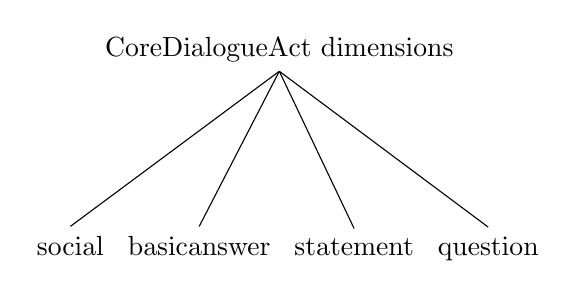
\begin{tikzpicture}
			\tikzset{every tree node/.style={align=center,anchor=base}}
			\tikzset{level 1+/.style={level distance=2\baselineskip}}
			\tikzset{frontier/.style={distance from root=6\baselineskip}}
			\Tree [.{CoreDialogueAct dimensions} social basicanswer statement question ]
		\end{tikzpicture}
	\end{center}
\end{frame}

\begin{frame}[fragile]
\frametitle{Social dimension}
	\begin{center}
		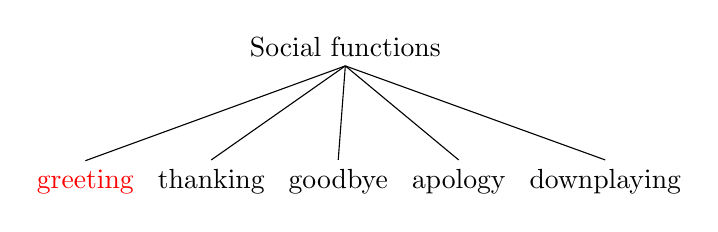
\begin{tikzpicture}
			\tikzset{every tree node/.style={align=center,anchor=base}}
			\tikzset{level 1+/.style={level distance=2\baselineskip}}
			\tikzset{frontier/.style={distance from root=4\baselineskip}}
			\Tree [.{Social functions} \node[color=red]{greeting}; thanking goodbye apology downplaying ]
		\end{tikzpicture}
	\end{center}
	\vspace{15pt}
	\begin{columns}
		\begin{column}{0.65\textwidth}
		{\color{teal} 
			\texttt{U: Good morning.}\\
			\vspace{10pt}
			\texttt{U: Nice to meet you.}\\
			\vspace{10pt}
			\texttt{U: Hello!}\\
		}
		\end{column}
		\begin{column}{0.35\textwidth}
			\footnotesize
			\texttt{CoreDialogueAct:} \\
				\vspace{10pt}
				$\begin{bmatrix}
						\texttt{Dimension:}    & \texttt{social}\\ 
						\texttt{Function:}     & \texttt{greeting}\\ 
				\end{bmatrix}$
		\end{column}
	\end{columns}
\end{frame}

\begin{frame}[fragile]
\frametitle{Social dimension}
	\begin{center}
		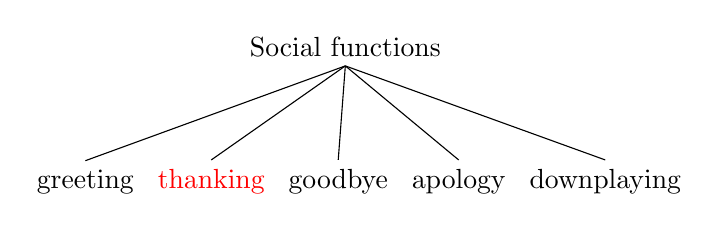
\begin{tikzpicture}
			\tikzset{every tree node/.style={align=center,anchor=base}}
			\tikzset{level 1+/.style={level distance=2\baselineskip}}
			\tikzset{frontier/.style={distance from root=4\baselineskip}}
			\Tree [.{Social functions} greeting \node[color=red]{thanking}; goodbye apology downplaying ]
		\end{tikzpicture}
	\end{center}
	\vspace{15pt}
	\begin{columns}
		\begin{column}{0.65\textwidth}
		{\color{teal} 
			\texttt{U: Thanks!}\\
			\vspace{10pt}
			\texttt{U: Thank you very much.}\\
			\vspace{10pt}
			\texttt{U: I'm so thankful!}\\
		}
		\end{column}
		\begin{column}{0.35\textwidth}
			\footnotesize
			\texttt{CoreDialogueAct:} \\
				\vspace{10pt}
				$\begin{bmatrix}
						\texttt{Dimension:}    & \texttt{social}\\ 
						\texttt{Function:}     & \texttt{thanking}\\ 
				\end{bmatrix}$
		\end{column}
	\end{columns}
\end{frame}

\begin{frame}[fragile]
\frametitle{Social dimension}
	\begin{center}
		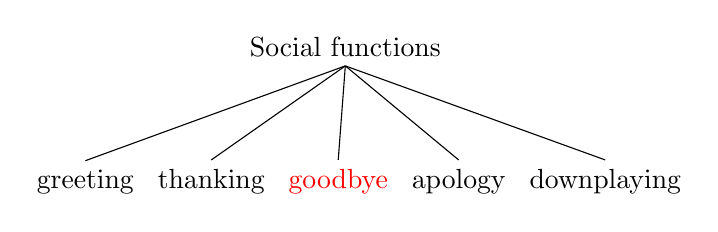
\begin{tikzpicture}
			\tikzset{every tree node/.style={align=center,anchor=base}}
			\tikzset{level 1+/.style={level distance=2\baselineskip}}
			\tikzset{frontier/.style={distance from root=4\baselineskip}}
			\Tree [.{Social functions} greeting thanking \node[color=red]{goodbye}; apology downplaying ]
		\end{tikzpicture}
	\end{center}
	\vspace{15pt}
	\begin{columns}
		\begin{column}{0.65\textwidth}
		{\color{teal} 
			\texttt{U: Have a good day!}\\
			\vspace{10pt}
			\texttt{U: See you later.}\\
			\vspace{10pt}
			\texttt{U: Bye!}\\
		}
		\end{column}
		\begin{column}{0.35\textwidth}
			\footnotesize
			\texttt{CoreDialogueAct:} \\
				\vspace{10pt}
				$\begin{bmatrix}
						\texttt{Dimension:}    & \texttt{social}\\ 
						\texttt{Function:}     & \texttt{goodbye}\\ 
				\end{bmatrix}$
		\end{column}
	\end{columns}
\end{frame}

\begin{frame}[fragile]
\frametitle{Social dimension}
	\begin{center}
		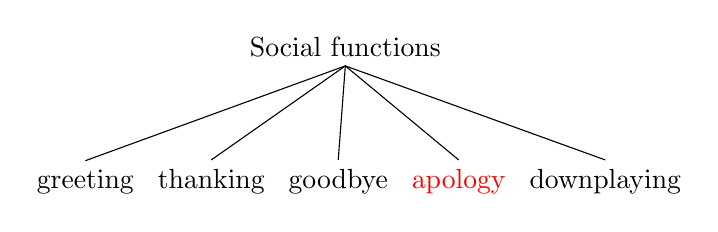
\begin{tikzpicture}
			\tikzset{every tree node/.style={align=center,anchor=base}}
			\tikzset{level 1+/.style={level distance=2\baselineskip}}
			\tikzset{frontier/.style={distance from root=4\baselineskip}}
			\Tree [.{Social functions} greeting thanking goodbye \node[color=red]{apology}; downplaying ]
		\end{tikzpicture}
	\end{center}
	\vspace{15pt}
	\begin{columns}
		\begin{column}{0.65\textwidth}
		{\color{teal} 
			\texttt{U: I'm sorry!}\\
			\vspace{10pt}
			\texttt{U: Excuse me.}\\
			\vspace{10pt}
			\texttt{U: My sincere apologies.}\\
		}
		\end{column}
		\begin{column}{0.35\textwidth}
			\footnotesize
			\texttt{CoreDialogueAct:} \\
				\vspace{10pt}
				$\begin{bmatrix}
						\texttt{Dimension:}    & \texttt{social}\\ 
						\texttt{Function:}     & \texttt{apology}\\ 
				\end{bmatrix}$
		\end{column}
	\end{columns}
\end{frame}


\begin{frame}[fragile]
\frametitle{Social dimension}
	\begin{center}
		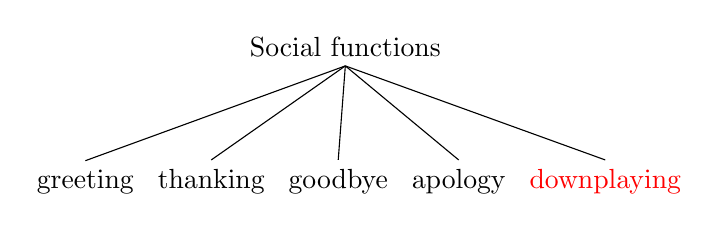
\begin{tikzpicture}
			\tikzset{every tree node/.style={align=center,anchor=base}}
			\tikzset{level 1+/.style={level distance=2\baselineskip}}
			\tikzset{frontier/.style={distance from root=4\baselineskip}}
			\Tree [.{Social functions} greeting thanking goodbye apology \node[color=red]{downplaying}; ]
		\end{tikzpicture}
	\end{center}
	\vspace{15pt}
	\begin{columns}
		\begin{column}{0.60\textwidth}
		{\color{teal} 
			\texttt{U: You're welcome!}\\
			\vspace{10pt}
			\texttt{U: Not at all.}\\
			\vspace{10pt}
			\texttt{U: Don't mention it.}\\
		}
		\end{column}
		\begin{column}{0.40\textwidth}
			\footnotesize
			\texttt{CoreDialogueAct:} \\
				\vspace{10pt}
				$\begin{bmatrix}
						\texttt{Dimension:}    & \texttt{social}\\ 
						\texttt{Function:}     & \texttt{downplaying}\\ 
				\end{bmatrix}$
		\end{column}
	\end{columns}
\end{frame}

\begin{frame}[fragile]
\frametitle{Basicanswer dimension}
	\begin{center}
		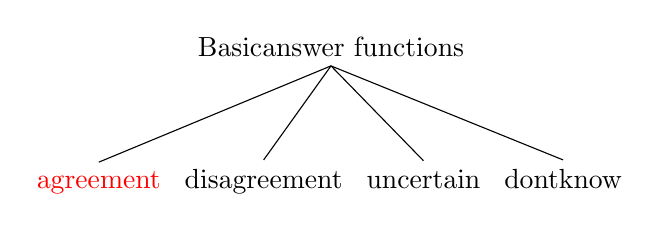
\begin{tikzpicture}
			\tikzset{every tree node/.style={align=center,anchor=base}}
			\tikzset{level 1+/.style={level distance=2\baselineskip}}
			\tikzset{frontier/.style={distance from root=4\baselineskip}}
			\Tree [.{Basicanswer functions} \node[color=red]{agreement}; disagreement uncertain dontknow ]
		\end{tikzpicture}
	\end{center}
	\vspace{15pt}
	\begin{columns}
		\begin{column}{0.60\textwidth}
		{\color{teal} 
			\texttt{U: Yes.}\\
			\vspace{10pt}
			\texttt{U: Ok.}\\
			\vspace{10pt}
			\texttt{U: That's right.}\\
		}
		\end{column}
		\begin{column}{0.40\textwidth}
			\footnotesize
			\texttt{CoreDialogueAct:} \\
				\vspace{10pt}
				$\begin{bmatrix}
						\texttt{Dimension:}    & \texttt{basicanswer}\\ 
						\texttt{Function:}     & \texttt{agreement}\\ 
				\end{bmatrix}$
		\end{column}
	\end{columns}
\end{frame}

\begin{frame}[fragile]
\frametitle{Basicanswer dimension}
	\begin{center}
		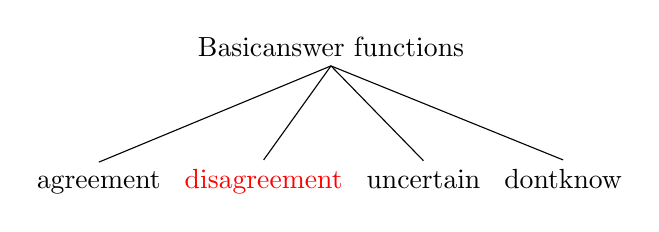
\begin{tikzpicture}
			\tikzset{every tree node/.style={align=center,anchor=base}}
			\tikzset{level 1+/.style={level distance=2\baselineskip}}
			\tikzset{frontier/.style={distance from root=4\baselineskip}}
			\Tree [.{Basicanswer functions} agreement \node[color=red]{disagreement}; uncertain dontknow ]
		\end{tikzpicture}
	\end{center}
	\vspace{15pt}
	\begin{columns}
		\begin{column}{0.58\textwidth}
		{\color{teal} 
			\texttt{U: No.}\\
			\vspace{10pt}
			\texttt{U: No way.}\\
			\vspace{10pt}
			\texttt{U: I can't agree.}\\
		}
		\end{column}
		\begin{column}{0.42\textwidth}
			\footnotesize
			\texttt{CoreDialogueAct:} \\
				\vspace{10pt}
				$\begin{bmatrix}
						\texttt{Dimension:}    & \texttt{basicanswer}\\ 
						\texttt{Function:}     & \texttt{disagreement}\\ 
				\end{bmatrix}$
		\end{column}
	\end{columns}
\end{frame}

\begin{frame}[fragile]
\frametitle{Basicanswer dimension}
	\begin{center}
		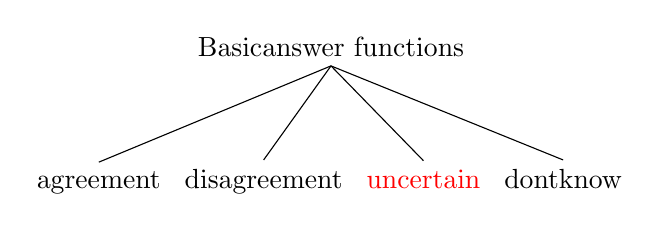
\begin{tikzpicture}
			\tikzset{every tree node/.style={align=center,anchor=base}}
			\tikzset{level 1+/.style={level distance=2\baselineskip}}
			\tikzset{frontier/.style={distance from root=4\baselineskip}}
			\Tree [.{Basicanswer functions} agreement disagreement \node[color=red]{uncertain}; dontknow ]
		\end{tikzpicture}
	\end{center}
	\vspace{15pt}
	\begin{columns}
		\begin{column}{0.60\textwidth}
		{\color{teal} 
			\texttt{U: Maybe.}\\
			\vspace{10pt}
			\texttt{U: Perhaps.}\\
			\vspace{10pt}
			\texttt{U: Probably.}\\
		}
		\end{column}
		\begin{column}{0.40\textwidth}
			\footnotesize
			\texttt{CoreDialogueAct:} \\
				\vspace{10pt}
				$\begin{bmatrix}
						\texttt{Dimension:}    & \texttt{basicanswer}\\ 
						\texttt{Function:}     & \texttt{uncertain}\\ 
				\end{bmatrix}$
		\end{column}
	\end{columns}
\end{frame}

\begin{frame}[fragile]
\frametitle{Basicanswer dimension}
	\begin{center}
		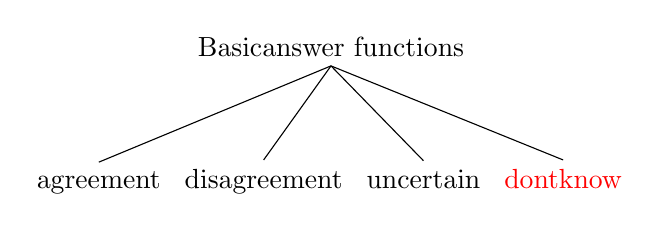
\begin{tikzpicture}
			\tikzset{every tree node/.style={align=center,anchor=base}}
			\tikzset{level 1+/.style={level distance=2\baselineskip}}
			\tikzset{frontier/.style={distance from root=4\baselineskip}}
			\Tree [.{Basicanswer functions} agreement disagreement uncertain \node[color=red]{dontknow}; ]
		\end{tikzpicture}
	\end{center}
	\vspace{15pt}
	\begin{columns}
		\begin{column}{0.60\textwidth}
		{\color{teal} 
			\texttt{U: I don't know.}\\
			\vspace{10pt}
			\texttt{U: I don't remember.}\\
			\vspace{10pt}
			\texttt{U: I have no idea.}\\
		}
		\end{column}
		\begin{column}{0.40\textwidth}
			\footnotesize
			\texttt{CoreDialogueAct:} \\
				\vspace{10pt}
				$\begin{bmatrix}
						\texttt{Dimension:}    & \texttt{basicanswer}\\ 
						\texttt{Function:}     & \texttt{dontknow}\\ 
				\end{bmatrix}$
		\end{column}
	\end{columns}
\end{frame}

\begin{frame}[fragile]
\frametitle{Statement dimension}
	\begin{center}
		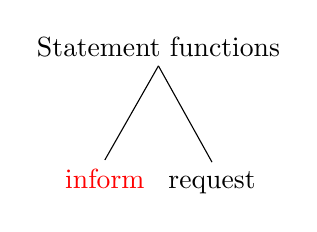
\begin{tikzpicture}
			\tikzset{every tree node/.style={align=center,anchor=base}}
			\tikzset{level 1+/.style={level distance=2\baselineskip}}
			\tikzset{frontier/.style={distance from root=4\baselineskip}}
			\Tree [.{Statement functions} \node[color=red]{inform}; request ]
		\end{tikzpicture}
	\end{center}
	\vspace{15pt}
	\begin{columns}
		\begin{column}{0.60\textwidth}
		{\color{teal} 
			\texttt{U: My name is ...}\\
			\vspace{10pt}
			\texttt{U: I live in ...}\\
			\vspace{10pt}
			\texttt{U: I don't want nothing else.}\\
		}
		\end{column}
		\begin{column}{0.40\textwidth}
			\footnotesize
			\texttt{CoreDialogueAct:} \\
				\vspace{10pt}
				$\begin{bmatrix}
						\texttt{Dimension:}    & \texttt{statement}\\ 
						\texttt{Function:}     & \texttt{inform}\\ 
				\end{bmatrix}$
		\end{column}
	\end{columns}
\end{frame}

\begin{frame}[fragile]
\frametitle{Statement dimension}
	\begin{center}
		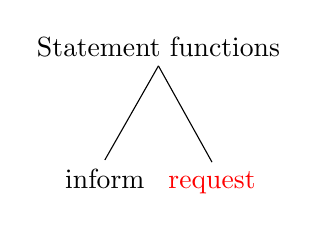
\begin{tikzpicture}
			\tikzset{every tree node/.style={align=center,anchor=base}}
			\tikzset{level 1+/.style={level distance=2\baselineskip}}
			\tikzset{frontier/.style={distance from root=4\baselineskip}}
			\Tree [.{Statement functions} inform \node[color=red]{request}; ]
		\end{tikzpicture}
	\end{center}
	\vspace{15pt}
	\begin{columns}
		\begin{column}{0.60\textwidth}
		{\color{teal} 
			\texttt{U: I want ...}\\
			\vspace{10pt}
			\texttt{U: I would need ...}\\
			\vspace{10pt}
			\texttt{U: Would you mind if ...?}\\
		}
		\end{column}
		\begin{column}{0.40\textwidth}
			\footnotesize
			\texttt{CoreDialogueAct:} \\
				\vspace{10pt}
				$\begin{bmatrix}
						\texttt{Dimension:}    & \texttt{statement}\\ 
						\texttt{Function:}     & \texttt{request}\\ 
				\end{bmatrix}$
		\end{column}
	\end{columns}
\end{frame}

\begin{frame}[fragile]
\frametitle{Question dimension}
	\begin{center}
		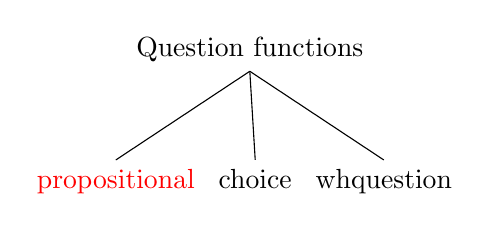
\begin{tikzpicture}
			\tikzset{every tree node/.style={align=center,anchor=base}}
			\tikzset{level 1+/.style={level distance=2\baselineskip}}
			\tikzset{frontier/.style={distance from root=4\baselineskip}}
			\Tree [.{Question functions} \node[color=red]{propositional}; choice whquestion ]
		\end{tikzpicture}
	\end{center}
	\vspace{15pt}
	\begin{columns}
		\begin{column}{0.58\textwidth}
		{\color{red} 
			\texttt{S: Do you agree with the date of the appointment?}\\}
			\vspace{10pt}
		{\color{teal} 
			\texttt{U: Do you like basketball?}\\
			\vspace{10pt}
			\texttt{U: Do you I am right?}\\
		}
		\end{column}
		\begin{column}{0.42\textwidth}
			\footnotesize
			\texttt{CoreDialogueAct:} \\
				\vspace{10pt}
				$\begin{bmatrix}
						\texttt{Dimension:}    & \texttt{question}\\ 
						\texttt{Function:}     & \texttt{propositional}\\ 
				\end{bmatrix}$
		\end{column}
	\end{columns}
\end{frame}

\begin{frame}[fragile]
\frametitle{Question dimension}
	\begin{center}
		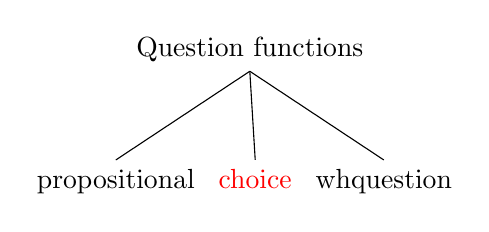
\begin{tikzpicture}
			\tikzset{every tree node/.style={align=center,anchor=base}}
			\tikzset{level 1+/.style={level distance=2\baselineskip}}
			\tikzset{frontier/.style={distance from root=4\baselineskip}}
			\Tree [.{Question functions} propositional \node[color=red]{choice}; whquestion ]
		\end{tikzpicture}
	\end{center}
	\vspace{15pt}
	\begin{columns}
		\begin{column}{0.60\textwidth}
		\small
		{\color{red} 
			\texttt{S: What do you want to do first, make a bank transfer or locate the nearest ATM?}\\
			\vspace{10pt}
			\texttt{S: Do you prefer coffee or tea?}\\
			\vspace{10pt}
			\texttt{S: When do you want the appointment, in the morning or in the afternoon?}\\
		}
		\end{column}
		\begin{column}{0.40\textwidth}
			\footnotesize
			\texttt{CoreDialogueAct:} \\
				\vspace{10pt}
				$\begin{bmatrix}
						\texttt{Dimension:}    & \texttt{question}\\ 
						\texttt{Function:}     & \texttt{choice}\\ 
				\end{bmatrix}$
		\end{column}
	\end{columns}
\end{frame}

\begin{frame}[fragile]
\frametitle{Question dimension}
	\begin{center}
		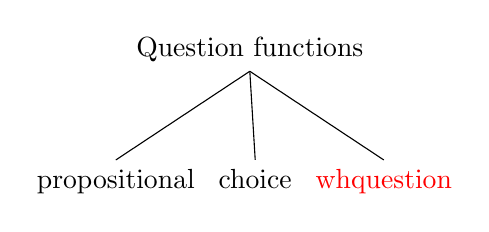
\begin{tikzpicture}
			\tikzset{every tree node/.style={align=center,anchor=base}}
			\tikzset{level 1+/.style={level distance=2\baselineskip}}
			\tikzset{frontier/.style={distance from root=4\baselineskip}}
			\Tree [.{Question functions} propositional choice \node[color=red]{whquestion}; ]
		\end{tikzpicture}
	\end{center}
	\vspace{15pt}
	\begin{columns}
		\begin{column}{0.60\textwidth}
		{\color{teal} 
			\texttt{U: What time is it?}\\
			\vspace{10pt}
			\texttt{U: How much is the doctor appointment?}\\
			\vspace{10pt}
			\texttt{U: Where is the nearest ATM?}\\
		}
		\end{column}
		\begin{column}{0.40\textwidth}
			\footnotesize
			\texttt{CoreDialogueAct:} \\
				\vspace{10pt}
				$\begin{bmatrix}
						\texttt{Dimension:}    & \texttt{question}\\ 
						\texttt{Function:}     & \texttt{whquestion}\\ 
				\end{bmatrix}$
		\end{column}
	\end{columns}
\end{frame}

\begin{frame}[fragile]
\frametitle{\texttt{TaskDialogueAct} structure}
	\begin{itemize}
		\item Dialogue act annotation is used to know the communicative function of user proferences.
		\item This doesn't depend on domain.
		\item But it lacks of semantic information. For example: In \texttt{statement-request} pair we wish to know what user wants to do and the object of his desire.
		\item This kind of information may depend on domain.
	\end{itemize}
	\scriptsize
	\pause
	\begin{lstlisting}[language=lekta]
classDef:StructureComplex ( 
	TaskDialogueAct : ( Action, Scope ) )

classDef:StructureBatch (	Action : ( ActionDomain ) )

classDef:ElementLiteral (	ActionDomain )
classDef:ElementLiteral (	Scope )
	\end{lstlisting}	
\end{frame}

\begin{frame}[fragile]
\frametitle{Domains implemented}
So we have implemented a couple of domains to do some testings:
	\setbeamercolor{block title}{use=structure,fg=white,bg=green!75!black}
	\setbeamercolor{block body}{use=structure,fg=black,bg=green!10!white}
	\begin{block}{Medical appointment}
		\begin{itemize}
			\item Task 1: \texttt{ActionDomain = `book'. Scope = `appointment'}
		\end{itemize}	
	\end{block}
	\pause
	\setbeamercolor{block title}{use=structure,fg=white,bg=green!75!black}
	\setbeamercolor{block body}{use=structure,fg=black,bg=green!10!white}
	\begin{block}{Banking management}
		\begin{itemize}
			\item Task 1: \texttt{ActionDomain = `consult'. Scope = `bankaccount'}
			\item Task 2: \texttt{ActionDomain = `locate'. Scope = `atm'}
			\item Task 3: \texttt{ActionDomain = `execute'. Scope = `transfer'}
		\end{itemize}
	\end{block}
\end{frame}

\begin{frame}[fragile]
\frametitle{Verb lemmas}
To detect actions in understanding stage, we associate some verbs lemmas to a certain action:
	\footnotesize
	\setbeamercolor{block title}{use=structure,fg=white,bg=green!75!black}
	\setbeamercolor{block body}{use=structure,fg=black,bg=green!10!white}
	\begin{block}{ActionDomain = `book'}
		book, establish, have, \textbf{make}, get, schedule, ask, set up, ...\\
		\vspace{10pt}
		{\color{teal} 
			\texttt{U: I want to get an appointment.}\\
			\texttt{U: I would like to make medical appointment.}\\
		}
	\end{block}
	\pause
	\footnotesize
	\setbeamercolor{block title}{use=structure,fg=white,bg=green!75!black}
	\setbeamercolor{block body}{use=structure,fg=black,bg=green!10!white}
	\begin{block}{ActionDomain = `execute'}
		\textbf{make}, move, execute, perform, do, accomplish, fulfill, effectuate, carry out, complete, ...\\
		\vspace{10pt}
		{\color{teal} 
			\texttt{U: I want to perform a bank transfer.}\\
			\texttt{U: I would like to make a transfer.}\\
		}
	\end{block}
	\pause
	Please note that a verb lemma can be associated with more than one \texttt{ActionDomain} (ambiguities everywhere!).
\end{frame}

\begin{frame}[fragile]
\frametitle{Parameters}
A `parameter' is some kind of useful information to complete a task. For example a \texttt{`datetime'} or an \texttt{`accountnumber'}.
\scriptsize
\begin{lstlisting}[language=lekta]
classDef:StructureComplex
(
	Parameter :
	(
		ParameterCategory, // 'terminal', 'and', 'or', ...
		ParameterType,     // 'datetime', 'accountnumber', ...
		ParameterValue,    // Similar to math expressions
		ParameterOperand1, 
		ParameterOperand2
	)
)
\end{lstlisting}
\pause
	\setbeamercolor{block title}{use=structure,fg=white,bg=green!75!black}
	\setbeamercolor{block body}{use=structure,fg=black,bg=green!10!white}
	\begin{block}{Example of \texttt{ParameterCategory}}
		{\color{teal} 
			\texttt{U: I want an appointment for tomorrow or the day after tomorrow.}\\
			\vspace{10pt}
			\texttt{U: My telephone numbers are 1234 and 5678.}\\
		}
	\end{block}
\end{frame}

\begin{frame}[fragile]
\frametitle{Parameters}
This information is provided by the user and may be compulsory ({\color{red}red}) or optative ({\color{teal}green})
	\scriptsize
	\setbeamercolor{block title}{use=structure,fg=white,bg=green!75!black}
	\setbeamercolor{block body}{use=structure,fg=black,bg=green!10!white}
	\begin{block}{Examples}
		\begin{itemize}
			\item \texttt{BookAppointment} task:
			\begin{itemize}
				\item \scriptsize{\color{red} \texttt{medicalspeciality}}
				\item \scriptsize{\color{red} \texttt{countryplace}}
				\item \scriptsize{\color{red} \texttt{phonenumber}}
				\item \scriptsize{\color{red} \texttt{peselnumber}} (Ok, it's a polish medical appointment!)
				\item \scriptsize{\color{teal} \texttt{datetime}}
			\end{itemize}
			\item \texttt{ConsultBankaccount} task: 
			\begin{itemize}
				\item \scriptsize{\color{red} \texttt{accountnumber}}
			\end{itemize}
			\item \texttt{LocateAtm} task: 
			\begin{itemize}
				\item \scriptsize{\color{red} \texttt{countryplace}}
			\end{itemize}
			\item \texttt{ExecuteTransfer} task: 
			\begin{itemize}
				\item \scriptsize{\color{red} \texttt{accountnumber}}
				\item \scriptsize{\color{red} \texttt{moneyamount}}
			\end{itemize}
		\end{itemize}
	\end{block}
\end{frame}

\begin{frame}[fragile]
\frametitle{Parameters classification}
\begin{itemize}
	\item Parameteres can be classified depending upon its domain. 
	\item If it's domain-independent we say that the parameter belongs to ``kernel'' domain.
	\item But take into account that we can move a parameter from its domain to kernel domain in order to make it \textbf{reusable}.
\end{itemize}
	\pause
	\setbeamercolor{block title}{use=structure,fg=white,bg=green!75!black}
	\setbeamercolor{block body}{use=structure,fg=black,bg=green!10!white}
	\begin{block}{Kernel domain implemented parameters}
	\begin{columns}
		\begin{column}{0.50\textwidth}
			\begin{itemize}
				\item \texttt{countryplace}
				\item \texttt{datetime}
				\item \texttt{letter}
				\item \texttt{moneyamount}
			\end{itemize}
		\end{column}
		\begin{column}{0.50\textwidth}
			\begin{itemize}
				\item \texttt{number}
				\item \texttt{ordinal}
				\item \texttt{phonenumber}
				\item \texttt{signchunk}
			\end{itemize}
		\end{column}
	\end{columns}
	\end{block}
\end{frame}
	
\begin{frame}[fragile]
\frametitle{Parameters classification}
	\setbeamercolor{block title}{use=structure,fg=white,bg=green!75!black}
	\setbeamercolor{block body}{use=structure,fg=black,bg=green!10!white}
	\begin{block}{Medical appointment domain implemented parameters}
		\begin{itemize}
			\item \texttt{medicalspeciality}
			\item \texttt{peselnumber}
		\end{itemize}
	\end{block}
	\setbeamercolor{block title}{use=structure,fg=white,bg=green!75!black}
	\setbeamercolor{block body}{use=structure,fg=black,bg=green!10!white}
	\begin{block}{Banking management domain implemented parameters}
		\begin{itemize}
			\item \texttt{accountnumber}
		\end{itemize}
	\end{block}
\end{frame}
	
\begin{frame}[fragile]
\frametitle{Parameters example: \texttt{datetime}}
\scriptsize
\begin{lstlisting}[language=lekta]
classDef:StructureComplex (
		DateTime: (
		BaseDate,
		OffsetDate,
		MinDate,
		MaxDate,
		GeneralTime
	)
)

classDef:StructureComplex (
		GeneralTime: (
		BaseTime,
		OffsetTime,
		MinTime,
		MaxTime
	)
)
\end{lstlisting}
\end{frame}
	
\begin{frame}[fragile]
\frametitle{Parameters example: \texttt{datetime}}
{\color{teal} 
	\texttt{U: Starting next thursday until 3pm to the day after 25 of august from noon to a quarter to nine in the afternoon.}\\
}
\pause
\vspace{15pt}
\scriptsize
\begin{lstlisting}[language=lekta]
(DateTime:
   (MinDate:(GeneralTime:(MaxTime:(BaseTime:(Hour:15))),
             OffsetDate :(DirectionOfTime:'forward',
                          Date           :(DayInWeek:4),
                          DayInWeekOffset:1)),
    MaxDate:(GeneralTime:(MinTime:(BaseTime:(Hour:12)),
                          MaxTime:(BaseTime:(Hour:20,
                                             Minute:45))),
             OffsetDate :(DirectionOfTime:'forward',
                          Date           :(Day:1)),
             BaseDate   :(Day  :25,
                          Month:8))))))
\end{lstlisting}
\end{frame}
	
\begin{frame}[fragile]
\frametitle{Parameters example: \texttt{countryplace}}
\scriptsize
\begin{lstlisting}[language=lekta]
classDef:StructureComplex ( 
		CountryPlace : (
		CountryName,
		CountryZone,
		CountryRegion,
		CountryProvince,
		CountryTown
	)
)

classDef:ElementLiteral (
	CountryName,
	CountryZone,
	CountryRegion,
	CountryProvince,
	CountryTown
)
\end{lstlisting}
\end{frame}

\begin{frame}[fragile]
\frametitle{Parameters example: \texttt{countryplace}}
{\small
\begin{itemize}
	\item We have used \textbf{NUTS} (Nomenclature of Territorial Units for Statistics) and \textbf{LAU} (Local Administrative Unit), two standards developed by European Union.
	\item We have, in the lexicon, all cities and towns of countries belonging to EU (except UK whose format file is different as usual!).
	\item This lexicon is expressed in the local language so we have Sevilla, but not Seville. We have Warszawa but not Warsaw.
\end{itemize}}
	\pause
	\scriptsize
	\setbeamercolor{block title}{use=structure,fg=white,bg=green!75!black}
	\setbeamercolor{block body}{use=structure,fg=black,bg=green!10!white}
	\begin{block}{Some examples}
	\begin{itemize}
		\item France: 39096 entries.
		\item Germany: 11167 entries.
		\item Bulgary: 10532 entries.
		\item Spain: 8837 entries.
		\item Italy: 8161 entries.
		\item Poland: 2478 entries. 
	\end{itemize}
	\end{block}
\end{frame}
	
\begin{frame}[fragile]
\frametitle{\texttt{DialogueAct} structure}
So we define this dialogue act type in Fluency:
\scriptsize
\begin{lstlisting}[language=lekta]
classDef:StructureComplex 
( 
 	DialogueAct :
  	(
		CoreDialogueAct,
		TaskDialogueAct,
		Parameters
	)
)	

classDef:StructureBatch
(
	Parameters :
	(
		Parameter
	)
)
\end{lstlisting}
\end{frame}
	

\begin{frame}[fragile]
\frametitle{Dialogue act annotation full example}
{\color{teal} 
	\texttt{U: I want to book an appointment for tomorrow to the dentist.}\\
}
\pause
\vspace{15pt}
\tiny
\begin{lstlisting}[language=lekta]
(DialogueAct:
   (CoreDialogueAct:(Dimension:'statement',
                     Function :'request')),
   (TaskDialogueAct:(Action:{(ActionDomain:'book')}
                     Scope:'appointment')),
   (Parameters:     {(Parameter:
                      (ParameterValue:
                       (DateTime:(OffsetDate:(DirectionOfTime:'forward',
                                              Date           :(Day:1))))),
                       ParameterCategory:'terminal',
                       ParameterType    :'datetime'),
                     (Parameter:
                      (ParameterValue:
                       (MedicalSpeciality:(SpecialityName:'Orthodontics'),
                       ParameterCategory:'terminal',
                       ParameterType    :'medicalspeciality')})
\end{lstlisting}
\end{frame}
				
\subsection{Fluency dialogue manager}

\begin{frame}
\frametitle{Script model}
\begin{itemize}
	\item Every task in all domains are modelled like scripts.
	\item A script consist of four parts:
	\begin{itemize}
	  \item \textbf{Descriptor:} Literal identificator to distingush this script among others.
		\item \textbf{Trigger:} Information that user must provide in order to activate the script.
		\item \textbf{InfoItems:} Place where the information is stored when script is activated. Can be provided by the user or the system itself.
		\item \textbf{Phases:} Subtasks needed to be performed in order to execute bigger one.
			\begin{itemize}
				\item Every phase has a priority level (0 the highest priority).
				\item Election mode: If all phases of level \emph{n} are finished we select a \emph{n+1} level phase randomly. 
			\end{itemize}
	\end{itemize}
	\item All scripts and states are stored in mindboard structures.
\end{itemize}
\end{frame}

\begin{frame}[fragile]
\frametitle{Script model: \texttt{ConsultBalance} script}
\scriptsize
\begin{lstlisting}[language=lekta]
Descriptor: 'ConsultBalance'

Trigger.CoreDialogueAct: ('statement', 'request')
Trigger.ActionDomain: 'consult' 
Trigger.Scope: 'bankaccount'
Trigger.Parameter: 'accountnumber'			
			
InfoItem.Parameter1: 'accountnumber' // Provided by the user
InfoItem.Parameter2: 'moneyamount' // Provided by the system
\end{lstlisting}

\tikzstyle{VertexStyle} = [shape            = rectangle,
                           minimum width    = 6ex,%
                           draw]
\tikzstyle{EdgeStyle}   = [->,>=stealth']      
\begin{center}
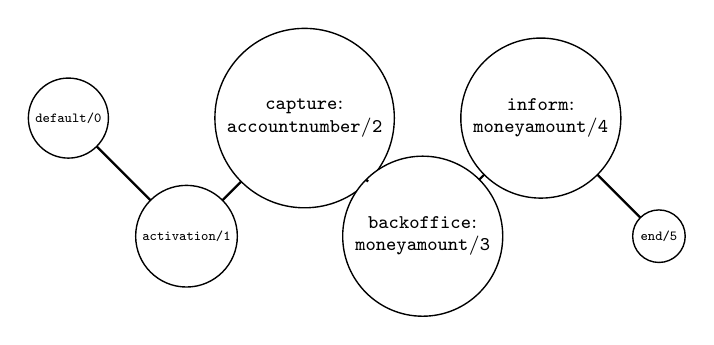
\begin{tikzpicture}[scale=1.0] 
	\SetGraphUnit{1.5} 
	\Vertex[L=\tiny\texttt{default/0}]{0} 	
		  \SOEA[L=\tiny\texttt{activation/1}](0){1}
			\NOEA[L=$\genfrac{}{}{0pt}{1}{\mathtt{capture:}}{\mathtt{accountnumber/2}}$](1){2}
			\SOEA[L=$\genfrac{}{}{0pt}{1}{\mathtt{backoffice:}}{\mathtt{moneyamount/3}}$](2){3}
			\NOEA[L=$\genfrac{}{}{0pt}{1}{\mathtt{inform:}}{\mathtt{moneyamount/4}}$](3){4}
      \SOEA[L=\tiny\texttt{end/5}](4){5}
  \Edges(0,1,2,3,4,5)
\end{tikzpicture}
\end{center}
\end{frame}

\begin{frame}[fragile]
\frametitle{Script model: \texttt{LocateAtm} script}
\scriptsize
\begin{lstlisting}[language=lekta]
Descriptor: 'LocateAtm'

Trigger.CoreDialogueAct: ('statement', 'request')
Trigger.ActionDomain: 'locate' 
Trigger.Scope: 'atm'
Trigger.Parameter: 'countryplace'			
			
InfoItem.Parameter1: 'countryplace' // Provided by the user
InfoItem.Parameter2: 'localization' // Provided by the system
\end{lstlisting}

\tikzstyle{VertexStyle} = [shape            = rectangle,
                           minimum width    = 6ex,%
                           draw]
\tikzstyle{EdgeStyle}   = [->,>=stealth']      
\begin{center}
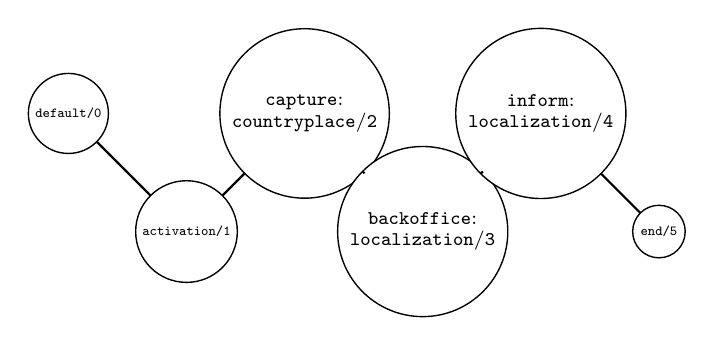
\begin{tikzpicture}[scale=1.0] 
	\SetGraphUnit{1.5} 
	\Vertex[L=\tiny\texttt{default/0}]{0} 	
		  \SOEA[L=\tiny\texttt{activation/1}](0){1}
			\NOEA[L=$\genfrac{}{}{0pt}{1}{\mathtt{capture:}}{\mathtt{countryplace/2}}$](1){2}
			\SOEA[L=$\genfrac{}{}{0pt}{1}{\mathtt{backoffice:}}{\mathtt{localization/3}}$](2){3}
			\NOEA[L=$\genfrac{}{}{0pt}{1}{\mathtt{inform:}}{\mathtt{localization/4}}$](3){4}
      \SOEA[L=\tiny\texttt{end/5}](4){5}
  \Edges(0,1,2,3,4,5)
\end{tikzpicture}
\end{center}
\end{frame}

\begin{frame}[fragile]
\frametitle{Script model: \texttt{MakeTransfer} script}
\scriptsize
\begin{lstlisting}[language=lekta]
Descriptor: 'MakeTransfer'

Trigger.CoreDialogueAct: ('statement', 'request')
Trigger.ActionDomain: 'execute' 
Trigger.Scope: 'transfer'
Trigger.Parameter1: 'accountnumber'			
Trigger.Parameter2: 'moneyamount'			
			
InfoItem.Parameter1: 'accountnumber' // Provided by the user
InfoItem.Parameter2: 'moneyamount'   // Provided by the user
\end{lstlisting}

\tikzstyle{VertexStyle} = [shape            = rectangle,
                           minimum width    = 6ex,%
                           draw]
\tikzstyle{EdgeStyle}   = [->,>=stealth']      
\begin{center}
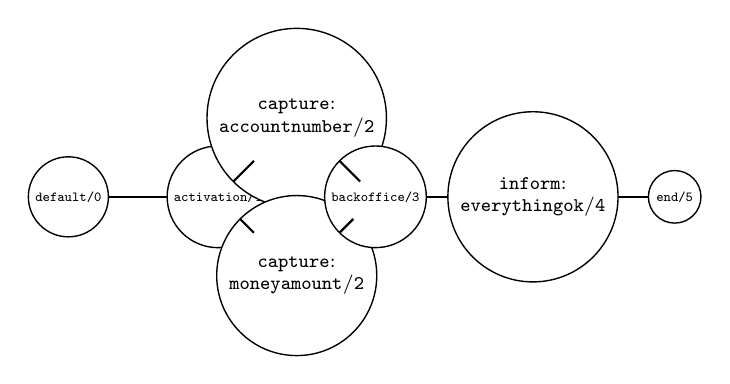
\begin{tikzpicture}[scale=1.0] 
	\SetGraphUnit{1.9} 
	\Vertex[L=\tiny\texttt{default/0}]{0} 	
		  \EA[L=\tiny\texttt{activation/1}](0){1}
			\SetGraphUnit{1} 
			\NOEA[L=$\genfrac{}{}{0pt}{1}{\mathtt{capture:}}{\mathtt{accountnumber/2}}$](1){2}
			\SOEA[L=$\genfrac{}{}{0pt}{1}{\mathtt{capture:}}{\mathtt{moneyamount/2}}$](1){6}
			\SOEA[L=\tiny\texttt{backoffice/3}](2){3}
			\SetGraphUnit{2.0} 
			\EA[L=$\genfrac{}{}{0pt}{1}{\mathtt{inform:}}{\mathtt{everythingok/4}}$](3){4}
			\SetGraphUnit{1.8} 
      \EA[L=\tiny\texttt{end/5}](4){5}
  \Edges(0,1,2,3,4,5)
	\Edges(1,6,3)
\end{tikzpicture}
\end{center}
\end{frame}


\begin{frame}[fragile]
\frametitle{Script model: \texttt{BookAppointment} script}
\scriptsize
\begin{lstlisting}[language=lekta]
Descriptor: 'BookAppointment'

Trigger.CoreDialogueAct: ('statement', 'request')
Trigger.ActionDomain: 'book' 
Trigger.Scope: 'appointment'
Trigger.Parameter1: 'medicalspeciality'			
Trigger.Parameter2: 'countryplace'			
Trigger.Parameter3: 'datetime'			
Trigger.Parameter4: 'phonenumber'			
Trigger.Parameter5: 'peselnumber'			

InfoItem.Parameter1: 'medicalspeciality' 
InfoItem.Parameter2: 'countryplace'      
InfoItem.Parameter3: 'datetime'          
InfoItem.Parameter4: 'phonenumber'       
InfoItem.Parameter5: 'peselnumber'       
\end{lstlisting}
\end{frame}

\begin{frame}[fragile]
\frametitle{Script model: \texttt{BookAppointment} script}
\scriptsize
\tikzstyle{VertexStyle} = [shape            = rectangle,
                           minimum width    = 6ex,%
                           draw]
\tikzstyle{EdgeStyle}   = [->,>=stealth']      
\begin{center}
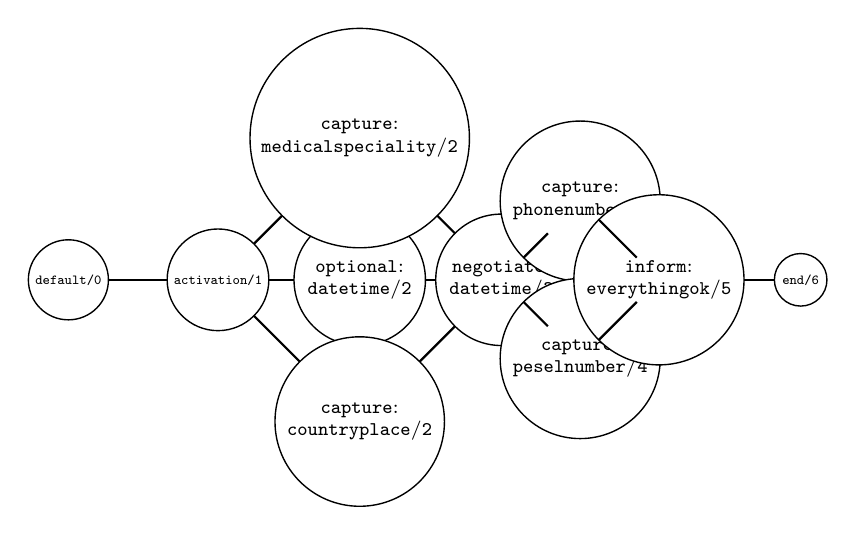
\begin{tikzpicture}[scale=1.0] 
	\SetGraphUnit{1.9} 
	\Vertex[L=\tiny\texttt{default/0}]{0} 	
		  \EA[L=\tiny\texttt{activation/1}](0){1}
			\SetGraphUnit{1.8} 
			\EA[L=$\genfrac{}{}{0pt}{1}{\mathtt{optional:}}{\mathtt{datetime/2}}$](1){2}
			\NOEA[L=$\genfrac{}{}{0pt}{1}{\mathtt{capture:}}{\mathtt{medicalspeciality/2}}$](1){3}
			\SOEA[L=$\genfrac{}{}{0pt}{1}{\mathtt{capture:}}{\mathtt{countryplace/2}}$](1){4}
			\EA[L=$\genfrac{}{}{0pt}{1}{\mathtt{negotiate:}}{\mathtt{datetime/3}}$](2){5}
			\SetGraphUnit{1.0} 
			\NOEA[L=$\genfrac{}{}{0pt}{1}{\mathtt{capture:}}{\mathtt{phonenumber/4}}$](5){6}
			\SOEA[L=$\genfrac{}{}{0pt}{1}{\mathtt{capture:}}{\mathtt{peselnumber/4}}$](5){7}
			\SOEA[L=$\genfrac{}{}{0pt}{1}{\mathtt{inform:}}{\mathtt{everythingok/5}}$](6){8}
			\SetGraphUnit{1.8} 
			\EA[L=\tiny\texttt{end/6}](8){9}
  \Edges(0,1,2,5,6)
	\Edges(1,3,5)
	\Edges(1,4,5)
	\Edges(5,7,8,9)
	\Edges(6,8)
\end{tikzpicture}
\end{center}
\end{frame}

\begin{frame}[fragile]
\frametitle{Fluency DM phases}
Every dialogue system turn execute this loop until last phase is reached:
\begin{enumerate}
	\item Start talking.
	\item Digest expectatives.
	\item Digest search scripts.
	\item Activate scripts.
	\item Select current script.
	\item Review states.
	\item Select current node.
	\item Process talking.
	\begin{enumerate}
		\item Execute node (go to 5).
		\item Wait node (go to 9).
	\end{enumerate}
	\item Close talking (go to 1 after user turn).
\end{enumerate}
\end{frame}

\begin{frame}[fragile]
\frametitle{Fluency DM phases}
	\setbeamercolor{block title}{use=structure,fg=white,bg=red!75!black}
	\setbeamercolor{block body}{use=structure,fg=black,bg=red!10!white}
	\begin{block}{1. Start talking}
	\begin{itemize}
		\item Erase output mindboard structures.
	\end{itemize}
	\end{block}
	\pause
	\setbeamercolor{block title}{use=structure,fg=white,bg=red!75!black}
	\setbeamercolor{block body}{use=structure,fg=black,bg=red!10!white}
	\begin{block}{2. Digest expectatives}
	\begin{itemize}
		\item Here we convert some parameters to the types of expected parameters.
		\item For example, if we are expecting a phone number and user says a number, we can transform on into the other.
	\end{itemize}
	\end{block}
	\pause
	\setbeamercolor{block title}{use=structure,fg=white,bg=red!75!black}
	\setbeamercolor{block body}{use=structure,fg=black,bg=red!10!white}
	\begin{block}{3. Digest search scripts}
	\begin{itemize}
		\item We analyze user proferences and create some triggering schemes.
		\item We give a scoring to every scheme to see its relevance.
	\end{itemize}
	\end{block}
\end{frame}

\begin{frame}[fragile]
\frametitle{Fluency DM phases}
	\footnotesize
	\setbeamercolor{block title}{use=structure,fg=white,bg=red!75!black}
	\setbeamercolor{block body}{use=structure,fg=black,bg=red!10!white}
	\begin{block}{4. Activate scripts}
	\begin{itemize}
		\item Depending on triggering schemes from previous phase we select what scripts must be activated.
		\item This is not trivial:
		\begin{itemize}
			\item What happens if comes a parameter from an active script, but not the current?
			\item What happens if comes a parameter from a non-active script?
			\item What happens if we have several triggered scripts with the same scoring?
		\end{itemize}
	\end{itemize}
	\end{block}
	\pause
	\footnotesize
	\setbeamercolor{block title}{use=structure,fg=white,bg=red!75!black}
	\setbeamercolor{block body}{use=structure,fg=black,bg=red!10!white}
	\begin{block}{5. Select current script}
	\begin{itemize}
		\item Previous phase ends sorting the activated scripts stack so we select, as current script, the one placed in the top of the stack.
		\item If we have a recently activated script it's the moment to recover some mid-term memory slots.
	\end{itemize}
	\end{block}
\end{frame}

\begin{frame}[fragile]
\frametitle{Fluency DM phases}
	\setbeamercolor{block title}{use=structure,fg=white,bg=red!75!black}
	\setbeamercolor{block body}{use=structure,fg=black,bg=red!10!white}
	\begin{block}{6. Review states}
	\begin{itemize}
		\item For every info item in the current script we review its state.
		\item For example, some of these states are:
		\begin{itemize}
				\item \textbf{empty}: The info item has no value.
				\item \textbf{proposed}: System has recently proposed the value of this item to the user.
				\item \textbf{checking}: We must check if the value of this item is valid and consistent.
				\item \textbf{captured}: We have recently captured this info item value from the user.
				\item \textbf{echoed}: This info item has been ``echoed'' to the user (implicit confirmation).
				\item \textbf{grounded}: User seems to agree with this info item.
				\item \textbf{recovered}: The value of this info item has been recently recovered from mid-term memory.
		\end{itemize}
	\end{itemize}
	\end{block}
\end{frame}

\begin{frame}[fragile]
\frametitle{Fluency DM phases}
	\small
	\setbeamercolor{block title}{use=structure,fg=white,bg=red!75!black}
	\setbeamercolor{block body}{use=structure,fg=black,bg=red!10!white}
	\begin{block}{7. Select current node}
	\begin{itemize}
		\item Here we select the next node to be executed in current script.
		\item Let $n$ the lowest priority level in script with not finished nodes.
		\item Select one of the not finished nodes with that priority level ramdonly.
	\end{itemize}
	\end{block}
	\pause
	\small
	\setbeamercolor{block title}{use=structure,fg=white,bg=red!75!black}
	\setbeamercolor{block body}{use=structure,fg=black,bg=red!10!white}
	\begin{block}{8. Process talking}
	\begin{itemize}
		\item If the selected node is an ``\textbf{execution}'' node, execute that node and go back to select current node stage.
		\item If the selected node is a ``\textbf{wait}'' node, we must pass the dialogue turn to user.
	\end{itemize}
	\end{block}
	\pause
	\small
	\setbeamercolor{block title}{use=structure,fg=white,bg=red!75!black}
	\setbeamercolor{block body}{use=structure,fg=black,bg=red!10!white}
	\begin{block}{9. Close talking}
	\begin{itemize}
		\item Erase input mindboard structures.
	\end{itemize}
	\end{block}

\end{frame}

\subsection{File and folder structure}

\begin{frame}
\frametitle{Main folder}
\dirtree{%
.1 {\color{blue}Fluency}.
.2 {\color{blue}Doc} {\color{teal} Some docs we have been generating}.
.2 {\color{blue}Kernel} {\color{teal} Generic domain}.
.2 {\color{blue}Domains} {\color{teal} Any other domain}.
.3 {\color{blue}Alter} {\color{teal} The union of next two domains}. 
.3 {\color{blue}BankingManagement}.
.3 {\color{blue}MedicalAppointments}.
.2 {\color{orange}AlterFluency.lkt} {\color{teal} Main project file}. 
.2 {\color{orange}EnglishAlterFluency.slk} {\color{teal} File for interpreter}.
}
	\pause
	\vspace{10pt}
	\setbeamercolor{block title}{use=structure,fg=white,bg=red!75!black}
	\setbeamercolor{block body}{use=structure,fg=black,bg=red!10!white}
	\begin{block}{Translation tip}
		There must be a \texttt{.slk} file for every language and every domain.
	\end{block}
\end{frame}

\begin{frame}
\frametitle{Domain folder example: Banking Management}
\scriptsize
\dirtree{%
.1 {\color{blue}BankingManagement}.
.2 {\color{blue}AccountNumber} {\color{teal} Parameter folder}.
.2 {\color{blue}Account} {\color{teal} Scope folder}.
.2 {\color{blue}ATM} {\color{teal} Scope folder}.
.2 {\color{blue}Transfer} {\color{teal} Scope folder}. 
.2 {\color{blue}Functions}.
.2 {\color{blue}Scripts}.
.2 {\color{orange}MainBankingManagementEnglishGeneration.lkt}. 
.2 {\color{orange}MainBankingManagementEnglishGrammar.lkt}.
.2 {\color{orange}MainBankingManagementEnglishLexicon.lkt}.
.2 {\color{orange}MainBankingManagementFunctions.lkt}.
.2 {\color{orange}MainBankingManagementTypes.lkt}.
}
	\pause
	\scriptsize
	\setbeamercolor{block title}{use=structure,fg=white,bg=red!75!black}
	\setbeamercolor{block body}{use=structure,fg=black,bg=red!10!white}
	\begin{block}{Translation tip}
		There must be three ``index'' files (grammar, lexicon and NLG) for every language.
	\end{block}
\end{frame}

\begin{frame}
\frametitle{Parameter folder example: Account Number}
\dirtree{%
.1 {\color{blue}AccountNumber}.
.2 {\color{blue}English}.
.3 {\color{blue}Generation}.
.4 {\color{orange}AccountNumberEnglishGeneration.lkt}.
.3 {\color{blue}Grammar}.
.4 {\color{orange}AccountNumberEnglishGrammar.lkt}.
.3 {\color{blue}Lexicon}.
.4 {\color{orange}AccountNumberEnglishLexicon.lkt}.
.2 {\color{blue}Functions}.
.3 {\color{orange}AccountNumberFunctions.lkt}.
.2 {\color{blue}Types}.
.3 {\color{orange}AccountNumberTypes.lkt} \small{\color{teal} Non-terminal symbols}.
.3 {\color{orange}LexicalAccountNumberTypes.lkt} \small{\color{teal} Terminal symbols}. 
.2 {\color{orange}MainAccountNumberTypes.lkt}. 
}
\end{frame}

\begin{frame}
\frametitle{Parameter folder example: Account Number}
	\scriptsize
	\setbeamercolor{block title}{use=structure,fg=white,bg=red!75!black}
	\setbeamercolor{block body}{use=structure,fg=black,bg=red!10!white}
	\begin{block}{Translation tip}
		There must be a folder for the three parts of the parameter (grammar, lexicon and NLG) for every language.
	\end{block}
	\pause
	\scriptsize
	\setbeamercolor{block title}{use=structure,fg=white,bg=blue!75!black}
	\setbeamercolor{block body}{use=structure,fg=black,bg=blue!10!white}
	\begin{block}{Parameter functions: \texttt{AccountNumberFunctions.lkt}}
		\begin{itemize}
			\item Possibilities of grouping for this parameter.
			\begin{itemize}
				\item \texttt{canMergeWithSequentialAccountNumber}. 
				\item \texttt{canMergeWithOrAccountNumber}.
				\item \texttt{canMergeWithAndAccountNumber}.
			\end{itemize}
			\item Valid formats for this parameters: \texttt{getParameterFormatsAccountNumber}.
			\item Additional checks not related with formats: \texttt{checkAccountNumberValidity}.
			\item Conversions from other parameters
			\begin{itemize}
				\item \texttt{convertNumberToAccountNumber}.
				\item \texttt{convertSignChunkToAccountNumber}.
				\item \texttt{...}
			\end{itemize}
		\end{itemize}
	\end{block}
\end{frame}

\begin{frame}[fragile]
	\setbeamercolor{block title}{use=structure,fg=white,bg=red!75!black}
	\setbeamercolor{block body}{use=structure,fg=black,bg=red!10!white}
	\begin{block}{Format example}
		\scriptsize
		\begin{lstlisting}[language=lekta]
ParameterFormats getParameterFormatsAccountNumber() {
	// Spanish account number
	ParameterFormats ret;
	ParameterFormat format;

	format <- '####################';
	BatchInsertEnd(ret, format);

	format <- 'es######################';
	BatchInsertEnd(ret, format);

	return ret;
}

/* Possible mask formats
#   Any valid number
^   Any letter 
@   Any letter or number
*   Anything */
		\end{lstlisting}
	\end{block}
\end{frame}

\begin{frame}[fragile]
	\setbeamercolor{block title}{use=structure,fg=white,bg=red!75!black}
	\setbeamercolor{block body}{use=structure,fg=black,bg=red!10!white}
	\begin{block}{\texttt{checkValidity} example: PESEL number}
		\tiny
		\begin{lstlisting}[language=lekta]
// https://en.wikipedia.org/wiki/PESEL

bool checkPeselNumberValidity( string pesel )
{
	int A <- ShapeToInt(LiteralPositionValue(pesel,1));
	int B <- ShapeToInt(LiteralPositionValue(pesel,2));
	int C <- ShapeToInt(LiteralPositionValue(pesel,3));
	int D <- ShapeToInt(LiteralPositionValue(pesel,4));
	int E <- ShapeToInt(LiteralPositionValue(pesel,5));
	int F <- ShapeToInt(LiteralPositionValue(pesel,6));
	int G <- ShapeToInt(LiteralPositionValue(pesel,7));
	int H <- ShapeToInt(LiteralPositionValue(pesel,8));
	int I <- ShapeToInt(LiteralPositionValue(pesel,9));
	int J <- ShapeToInt(LiteralPositionValue(pesel,10));
	int K <- ShapeToInt(LiteralPositionValue(pesel,11));

	int weighted <- 1*A + 3*B + 7*C + 9*D + 1*E + 3*F + 7*G + 9*H + 1*I + 3*J;
	int remainder <- Modulo(weighted, 10);
	int complement <- Modulo(10 - remainder, 10);

	if(complement != K)	
		return False;
	
	return True;
}
		\end{lstlisting}
	\end{block}
\end{frame}

\begin{frame}
\frametitle{Scope folder example: ATM}
\dirtree{%
.1 {\color{blue}ATM}.
.2 {\color{blue}English}.
.3 {\color{blue}Grammar}.
.4 {\color{orange}ATMEnglishGrammar.lkt}.
.3 {\color{blue}Lexicon}.
.4 {\color{orange}ATMEnglishLexicon.lkt}.
.2 {\color{blue}Types}.
.3 {\color{orange}ATMTypes.lkt}.
.3 {\color{orange}LexicalATMTypes.lkt}. 
.2 {\color{orange}MainATMTypes.lkt}. 
}
	\pause
	\vspace{10pt}
	\setbeamercolor{block title}{use=structure,fg=white,bg=red!75!black}
	\setbeamercolor{block body}{use=structure,fg=black,bg=red!10!white}
	\begin{block}{Translation tip}
		Again \texttt{English} folder structure must be replicated in other languages.
	\end{block}
\end{frame}

\begin{frame}
\frametitle{Scripts folder example: Banking Management}
\dirtree{%
.1 {\color{blue}Scripts}.
.2 {\color{blue}English}.
.3 {\color{orange}BankingManagementEnglishGeneration.lkt}.
.2 {\color{orange}BankingManagementScripts.lkt} {\color{teal} Functions generating the scripts of this domain}. 
}
	\pause
	\vspace{10pt}
	\setbeamercolor{block title}{use=structure,fg=white,bg=red!75!black}
	\setbeamercolor{block body}{use=structure,fg=black,bg=red!10!white}
	\begin{block}{Translation tip}
		File in \texttt{English} folder has some natural language generation rules related with the scripts.
	\end{block}
\end{frame}

\begin{frame}[fragile]
\frametitle{Functions folder example: Banking Management}
\dirtree{%
.1 {\color{blue}Functions}.
.2 {\color{orange}BankingManagementBackOffice.lkt}  {\color{teal} Back office callback functions}.
.2 {\color{orange}BankingManagementFunctions.lkt} {\color{teal} Functions related with current domain}. 
}
\end{frame}

\begin{frame}[fragile]
\frametitle{Functions folder example: Banking Management}
	\setbeamercolor{block title}{use=structure,fg=white,bg=red!75!black}
	\setbeamercolor{block body}{use=structure,fg=black,bg=red!10!white}
	\begin{block}{Translation tip}
	Among other functions, we have to link lemmas with actions:
		\tiny
		\begin{lstlisting}[language=lekta]
string getActionDomainFromLemmaBankingManagement(string lemma)
{
	switch (lemma) 
	{
		// Action consult (scope: 'bankaccount')
		case 'consult'   { return 'consult'; }
		case 'check'     { return 'consult'; }
		
		// Action locate (scope: 'atm')
		case 'locate'    { return 'locate'; }
		case 'look for'  { return 'locate'; }
		case 'search'    { return 'locate'; }
		case 'find'      { return 'locate'; }

		// Action execute (scope: 'transfer')
		case 'make'      { return 'execute'; }
		case 'perform'   { return 'execute'; }
		case 'fulfill'   { return 'execute'; }
		case 'complete'  { return 'execute'; }
	}

	return 'unknown';
}
		\end{lstlisting}
	\end{block}
\end{frame}

\begin{frame}[fragile]
\frametitle{Kernel folder}
\scriptsize
\dirtree{%
.1 {\color{blue}Kernel}.
.2 {\color{blue}CountryPlace} {\color{teal} Parameter folder}. 
.2 {\color{blue}...}. 
.2 {\color{blue}Social} {\color{teal} Core dialogue act folder}.
.2 {\color{blue}...}. 
.2 {\color{blue}Generation} {\color{teal} Generation rules for kernel scripts}.
.2 {\color{blue}Generic} {\color{teal} Generic natural language features}.
.2 {\color{blue}Constants} {\color{teal} Some useful lekta constants}. 
.2 {\color{blue}DialogueManager} {\color{teal} DM implementation}.
.2 {\color{blue}Macros} {\color{teal} Lekta macros for verbs and nouns inflections}.
.2 {\color{orange}MainEnglishGeneration.lkt}. 
.2 {\color{orange}MainEnglishGrammar.lkt}.
.2 {\color{orange}MainEnglishLexicon.lkt}.
.2 {\color{orange}MainFunctions.lkt}.
.2 {\color{orange}MainTypes.lkt}.
}
\end{frame}

\begin{frame}[fragile]
\frametitle{Core dialogue act folder example: Social}
\footnotesize
\dirtree{%
.1 {\color{blue}Social}.
.2 {\color{blue}English} {\color{red} Translation tip!}. 
.3 {\color{blue}Generation}. 
.4 {\color{orange}GenerationSocialGoodbye.lkt}.
.4 {\color{orange}GenerationSocialGreeting.lkt}.
.3 {\color{blue}Grammar}. 
.4 {\color{orange}SocialEnglishGrammar.lkt}.
.3 {\color{blue}Lexicon}. 
.4 {\color{orange}SocialEnglishLexicon.lkt}.
.2 {\color{blue}Types}. 
.3 {\color{orange}LexicalSocialTypes.lkt}.
.3 {\color{orange}SocialTypes.lkt}.
.2 {\color{orange}MainSocialTypes.lkt}.
}
\end{frame}

\begin{frame}[fragile]
\frametitle{Generation folder}
\dirtree{%
.1 {\color{blue}Generation}.
.2 {\color{blue}English} {\color{red} Translation tip!}. 
.3 {\color{orange}GenerationDisambiguatorKernel.lkt}.
.3 {\color{orange}GenerationKernel.lkt}.
.2 {\color{blue}Functions}. 
.3 {\color{orange}GenerationFunctions.lkt}.
}		
\end{frame}

\begin{frame}[fragile]
\frametitle{Generic folder}
\footnotesize
\dirtree{%
.1 {\color{blue}Generic}.
.2 {\color{blue}English} {\color{red} Translation tip!}. 
.3 {\color{blue}Grammar}.
.4 {\color{orange}GenericEnglishGrammar.lkt}.
.3 {\color{blue}Lexicon}.
.4 {\color{orange}GenericEnglishLexicon.lkt}.
.4 {\color{orange}NounsEnglishLexicon.lkt}.
.4 {\color{orange}VerbsEnglishLexicon.lkt}.
.2 {\color{blue}Functions}. 
.3 {\color{orange}FormatFunctions.lkt}.
.3 {\color{orange}GenericFunctions.lkt}.
.2 {\color{blue}Types}. 
.3 {\color{orange}GenericTypes.lkt}.
.3 {\color{orange}FormatTypes.lkt}.
.3 {\color{orange}LexicalGenericTypes.lkt}.
}		
\end{frame}

\section{Functional analysis}

\begin{frame}
\end{frame}



\end{document}

	


